\documentclass[11pt,letterpaper]{article}

% Essential packages
\usepackage[utf8]{inputenc}
\usepackage[T1]{fontenc}
\usepackage[margin=1in]{geometry}
\usepackage{fancyhdr}
\usepackage{graphicx}
\usepackage{float}

% Math packages
\usepackage{amsmath}
\usepackage{amsfonts}
\usepackage{amssymb}
\usepackage{amsthm}

% Table packages
\usepackage{booktabs}
\usepackage{array}
\usepackage{tabularx}
\usepackage{longtable}

% List packages
\usepackage{enumitem}
\usepackage{float}

% Graphics and plotting
\usepackage{tikz}
\usepackage{pgfplots}
\pgfplotsset{compat=1.18}
\usepackage{subcaption}

% Citation and references
\usepackage[round,authoryear]{natbib}
\usepackage{url}

% Code listings and algorithms
\usepackage{listings}
\usepackage{xcolor}
\usepackage{algorithm}
\usepackage[noend]{algpseudocode}

% Configure code listings for Python
\lstset{
    language=Python,
    basicstyle=\ttfamily\small,
    keywordstyle=\color{blue},
    commentstyle=\color{gray},
    stringstyle=\color{red},
    showstringspaces=false,
    breaklines=true,
    frame=single,
    numbers=left,
    numberstyle=\tiny\color{gray},
    captionpos=b
}

% Hyperlinks (load last)
\usepackage[colorlinks=true,linkcolor=blue,citecolor=blue,urlcolor=blue]{hyperref}

% Custom commands for common actuarial notation
\newcommand{\E}{\mathbb{E}}
\newcommand{\Var}{\text{Var}}
\newcommand{\Cov}{\text{Cov}}
\newcommand{\Prob}{\mathbb{P}}

% Header and footer setup
\pagestyle{fancy}
\fancyhf{}
\fancyhead[L]{Ergodicity Simulation Framework for Insurance}
\fancyhead[R]{}
\fancyfoot[C]{\thepage}

% Title page information
\title{\Large \textbf{Ergodicity Economics in Property \& Casualty Insurance: \\
A Simulation Framework for Understanding Risk Appetite}}

\author{Alex Filiakov, ACAS\\
\texttt{alexfiliakov@gmail.com}}

\date{\today}

\begin{document}

\maketitle

\begin{abstract}
This white paper introduces a new simulation framework based on ergodicity economics principles for analyzing insurance risk appetite in Property \& Casualty markets. Traditional ensemble-based risk models may not adequately capture the temporal dynamics of insurance company decision-making. This introductory paper demonstrates that insurance appetite varies significantly with company size, measured by capitalization and revenue.
\\\\
\textbf{Keywords:} ergodicity economics, insurance appetite, risk modeling, simulation framework
\end{abstract}

\newpage
\tableofcontents
\newpage

\section{Executive Summary}

This section should provide a concise overview of the entire paper, typically 1-2 pages covering:
\begin{itemize}
    \item The problem addressed
    \item Your key methodology (simulation framework)
    \item Primary finding about company size and insurance appetite
    \item Practical implications for the industry
\end{itemize}

% TODO: Complete executive summary content

\section{Introduction}

\subsection{Current Challenges in Insurance Appetite Modeling}

Traditional approaches to modeling insurance appetite in P\&C markets face several limitations:
\begin{itemize}
    \item Reliance on ensemble averages rather than temporal sequences
    \item Inadequate consideration of path-dependent effects
    \item Limited incorporation of company-specific factors
\end{itemize}

\subsection{The Promise of Ergodicity Economics}

Ergodicity economics, developed by \citet{peters2025ergodicity}, offers a new perspective on decision-making under uncertainty. Unlike traditional expected utility theory, which focuses on ensemble averages, ergodicity economics emphasizes the importance of time averages and growth rates.

% TODO: Add more detailed introduction content

\section{Theoretical Foundation}

\subsection{Ergodicity vs. Non-Ergodicity in Financial Systems}

The distinction between time averages and ensemble averages lies at the heart of ergodic economics, a framework pioneered by \citet{peters2019ergodicity} that challenges fundamental assumptions in economic theory. A stochastic process is ergodic if its time average equals its ensemble average:

\begin{equation}
\lim_{T \to \infty} \frac{1}{T} \int_0^T f(X_t) dt = \E[f(X)]
\end{equation}

For ergodic systems, what happens to an individual over time matches the average across many individuals at a single point in time. However, most economic processes violate this equality, creating a fundamental divergence between individual experience and statistical expectations.

The ensemble average represents the expected value across many parallel scenarios:
\begin{equation}
\langle W \rangle = \E[W_t] = \frac{1}{N} \sum_{i=1}^{N} W_i(t)
\end{equation}

where $W_i(t)$ represents the wealth of entity $i$ at time $t$. This is the traditional expected value used in most economic and actuarial analysis.

In contrast, the time average captures what a single entity experiences over its lifetime:
\begin{equation}
g_{\text{time}} = \lim_{T \to \infty} \frac{1}{T} \ln\left(\frac{W_T}{W_0}\right)
\end{equation}

For multiplicative processes with uncertainty, Jensen's inequality ensures these two averages diverge systematically, with profound implications for insurance and risk management \citep{peters2016evaluating}. Jensen's inequality states that for a random variable $W$ and a convex function $f$:

\begin{equation}
f(\E[W]) \leq \E[f(W)]
\end{equation}

In the context of multiplicative wealth dynamics, this means that the expected growth rate (ensemble average) can be misleadingly optimistic compared to the actual growth experienced over time (time average).

\subsection{Insurance Markets as Non-Ergodic Systems}

Insurance markets exhibit fundamentally non-ergodic properties that invalidate traditional expected value analysis. The non-ergodicity arises from several structural features:

\textbf{Multiplicative Wealth Dynamics:} Corporate wealth evolves through multiplicative processes where returns compound on existing capital:
\begin{equation}
W_{t+1} = W_t \cdot (1 + r_t - l_t)
\end{equation}
where $r_t$ represents returns and $l_t$ represents proportional losses. This multiplicative structure means that the order and magnitude of losses matter critically. For example, a 50\% loss followed by a 50\%~gain leaves wealth at 75\% of its original value, not 100\%.

\textbf{Absorbing Bankruptcy Barrier:} Once a company reaches zero equity (bankruptcy), it cannot recover:
\begin{equation}
W_t = 0 \Rightarrow W_{t+k} = 0 \quad \forall k > 0
\end{equation}
This absorbing barrier creates fundamental asymmetry: while gains are unbounded, losses are limited to -100\%. The existence of this barrier means that time averages systematically underperform ensemble averages.

\textbf{Path-Dependent Capital Requirements:} Regulatory and market constraints depend on the entire history of losses and capital positions, not just current values. A company that experienced large losses faces higher capital costs and restricted growth opportunities, even after recovering to its original capital level.

\textbf{Finite Decision Horizons:} While ensemble averages assume infinite repeated trials, real companies operate with finite time horizons constrained by management tenure, regulatory cycles, and strategic planning periods. Over finite horizons, the divergence between time and ensemble averages can be substantial.

These non-ergodic features explain why insurance appears valuable even when premiums substantially exceed expected losses. The relevant metric is not the ensemble average (expected value) but the time average (growth rate) \citep{peters2011time}.

\subsection{Mathematical Framework}

Consider a company with wealth $W_t$ evolving under stochastic dynamics. In the absence of insurance, wealth follows:
\begin{equation}
W_{t+1} = W_t \cdot \left(1 + \mu - \sigma Z_t - L_t\right)
\end{equation}

where:
\begin{itemize}
    \item $\mu$ is the drift (expected return from operations)
    \item $\sigma Z_t$ represents operational volatility with $Z_t \sim \mathcal{N}(0,1)$
    \item $L_t$ represents catastrophic losses occurring with frequency $\lambda$ and severity distribution $F_L$
\end{itemize}

The time-average growth rate without insurance is:
\begin{equation}
g_{\text{uninsured}} = \mu - \frac{\sigma^2}{2} - \lambda \cdot \E\left[\ln\left(1 - \frac{L}{W}\right)\right]
\end{equation}

The first two terms represent the familiar geometric Brownian motion result, while the third term captures the impact of jump losses. Note the appearance of $\E[\ln(1 - L/W)]$ rather than $\E[L/W]$—this logarithmic transformation is crucial and explains why losses have a disproportionate impact on growth.

With insurance featuring deductible $D$ and premium rate $\pi$, the growth rate becomes:
\begin{equation}
g_{\text{insured}} = \mu - \frac{\sigma^2}{2} - \pi - \lambda \cdot \E\left[\ln\left(1 - \frac{\min(L, D)}{W}\right)\right]
\end{equation}

The insurance creates value when:
\begin{equation}
g_{\text{insured}} > g_{\text{uninsured}}
\end{equation}

This inequality can hold even when $\pi > \lambda \cdot \E[L]$ (premium exceeds expected losses), particularly for companies with:
\begin{itemize}
    \item Lower capital levels (higher $L/W$ ratios)
    \item Higher operational leverage (larger $\mu$ potential)
    \item Greater loss severity risk (heavy-tailed $F_L$)
\end{itemize}

The optimal insurance strategy maximizes time-average growth, not expected wealth. This leads naturally to the Kelly criterion \citep{kelly1956new}, which in the insurance context becomes:
\begin{equation}
D^* = \arg\max_D \E\left[\ln\left(\frac{W_{t+1}}{W_t}\right)\right]
\end{equation}

This optimization framework explains the simulation results showing that smaller companies optimally choose lower deductibles despite higher relative premium costs: they face greater proportional impact from losses and thus benefit more from variance reduction.

\textbf{Special Case: Deterministic Operations.} The framework simplifies elegantly when operational volatility is zero ($\sigma = 0$), as in this simulation. The growth rates become:
\begin{align}
g_{\text{uninsured}} &= \mu - \lambda \cdot \E\left[\ln\left(1 - \frac{L}{W}\right)\right] \\
g_{\text{insured}} &= \mu - \pi - \lambda \cdot \E\left[\ln\left(1 - \frac{\min(L,D)}{W}\right)\right]
\end{align}

Even without operational volatility, insurance creates value because losses themselves introduce multiplicative volatility. The insurance value condition becomes:
\begin{equation}
\lambda \cdot \E\left[\ln\left(\frac{1 - \min(L,D)/W}{1 - L/W}\right)\right] > \pi
\end{equation}

This expression is positive whenever losses exceed the deductible, demonstrating that insurance enhances growth by capping catastrophic losses—converting unpredictable large losses into predictable premium costs. The absence of operational volatility actually clarifies the pure insurance value proposition: reducing the multiplicative impact of tail risks on long-term growth rates.

\section{Simulation Framework Overview}

\subsection{Architecture and Key Components}

The simulation framework implements a comprehensive ergodic analysis system that bridges corporate finance, insurance economics, and stochastic modeling. Rather than treating insurance as a simple expected value calculation, the framework captures the fundamental non-ergodicity of business growth under uncertainty.

\subsubsection{Framework Design Philosophy}

The architecture centers on a critical distinction from traditional actuarial models: it compares time-average growth rates (what a single company experiences over its lifetime) with ensemble-average growth rates (statistical expectations across many parallel scenarios). This ergodic economics approach, pioneered by \citet{peters2019ergodicity}, reveals that insurance can enhance growth even when premiums substantially exceed expected losses, a result invisible to traditional expected value analysis.

The framework employs Monte Carlo simulation to generate thousands of independent business trajectories, each experiencing unique sequences of loss events. By tracking individual path dynamics, the system quantifies the lift in time-average growth rate offered by insurance in certain business scenarios.

\subsubsection{Corporate Business Model}

At the framework's core lies an illustrative manufacturing company with realistic financial dynamics. The model tracks complete corporate accounting relationships while maintaining computational efficiency for large-scale simulations.

Revenue generation follows an asset turnover model where annual revenues equal total assets multiplied by an asset turnover ratio (typically 0.8 to 1.2). This approach naturally scales business activity with company size while allowing exploration of capital efficiency effects. Operating income derives from revenues through configurable operating margins, capturing the fundamental profitability before considering loss events.

The income statement dynamics incorporate operating revenues, margins, claim losses, insurance premiums, and corporate taxes. Critically, revenues serve as the exposure base for loss generation, creating a direct link between business scale and risk exposure. Premiums are calibrated at the outset, assuming accurate matching to the expected loss distribution, and loaded for costs to a realistic target loss ratio. Premiums are subsequently scaled with revenues, in line with the underlying loss exposure base. After-tax earnings flow to retained earnings, driving balance sheet growth absent external capital raises.

Balance sheet evolution tracks assets, liabilities, and equity through time, maintaining the fundamental accounting equation. When losses are incurred, they follow a 10-year payment schedule, reflecting typical commercial insurance claim settlement patterns. The company's portion (deductible amount) requires immediate collateral via letter of credit. The collateral accrues at market rates and is gradually released as claim payments are made over the years. Insurance recoveries are tracked as receivables, but have no practical effect on the company as insurer defaults are not modeled.

\subsubsection{Loss Generation Module}

The framework implements a three-tier loss structure that captures the full spectrum of business risks:

\textbf{Attritional losses} represent high-frequency, low-severity events such as minor operational disruptions, small liability claims, or routine equipment failures. These follow a compound Poisson process with lognormal severities, creating a steady baseline loss burden.

\textbf{Large losses} capture moderate-frequency events with more substantial impact, such as significant liability claims, major equipment breakdowns, or supply chain disruptions. These also follow a compound Poisson-lognormal structure but with parameters shifted toward less frequent, more severe events.

\textbf{Catastrophic losses} model low-probability, high-impact events that can threaten business continuity, such as natural disasters, major litigation, or systemic failures. These events, while rare, fundamentally alter growth trajectories, erode capital, and drive much of the insurance value proposition. Poisson-Pareto distributions capture the heavy-tailed nature of these risks.

Each loss type draws from distinct frequency and severity distributions, with all claim counts scaled by revenue exposure. Claim correlations are not modeled.

\subsubsection{Insurance Mechanism}

The insurance module focuses on deductible optimization, the primary decision variable for most corporate insurance programs. While the framework supports complex insurance towers with multiple attachment points, coverage types and limits, for this first experiment, the configuration was simplified with virtually unlimited coverage. These high coverage limits effectively eliminate ruin risk, isolating the deductible's impact on growth dynamics.

For each loss event, the model determines payment allocation between the company (up to the deductible) and insurers (excess of deductible). Premium calculations incorporate expected losses, expense loadings, and risk charges, with pricing that reflects realistic market conditions rather than actuarially fair rates. Again, for this first experiment, the pricing was simplified to a single target loss ratio, with no risk loadings or insurance cycle dynamics. Future work will explore more sophisticated pricing models.

\subsubsection{Ergodic Analysis Engine}

The framework's analytical core computes and compares growth metrics across insured and uninsured scenarios, revealing the ergodic effects of insurance.

The time-average growth rate for each trajectory is calculated as:
\begin{equation}
g_{\text{time}} = \frac{1}{T} \ln\left(\frac{W_T}{W_0}\right)
\end{equation}
where $W_T$ represents terminal wealth (equity) and $W_0$ initial wealth. This logarithmic formulation captures the multiplicative nature of business growth, where percentage changes compound over time.

Growth lift quantifies insurance value as the difference between insured and uninsured time-average growth rates:
\begin{equation}
\text{Growth Lift} = g_{\text{time}}^{\text{insured}} - g_{\text{time}}^{\text{uninsured}}
\end{equation}

Positive growth lift indicates that insurance enhances long-term wealth accumulation despite premium costs.

The framework distinguishes between survival optimization (avoiding ruin) and growth optimization (maximizing wealth accumulation). While high coverage limits virtually eliminate bankruptcy risk in the modeled scenarios, different deductible levels create a trade-off between premium costs and retained volatility that affects growth rates. The optimal deductible maximizes time-average growth rather than merely ensuring survival.

\subsubsection{Parameter Interactions}

The simulation explores a multidimensional parameter space that captures key drivers of insurance appetite:

\textbf{Capitalization levels} (\$5M, \$10M, \$25M) represent different company sizes, with smaller firms facing proportionally larger impacts from individual losses. This size effect proves central to understanding why optimal deductibles vary across companies. At retentions beyond \$25M and with the loss distribution unaltered, full retention becomes optimal (i.e., no insurance) as loss volatility relative to capital diminishes, so these higher capitalization levels were removed from consideration.

\textbf{Asset turnover ratios} (0.8 to 1.2) capture capital efficiency, with higher ratios generating more revenue (and thus more loss exposure) per dollar of assets.

\textbf{Operating margins} determine profitability buffers against losses. Higher-margin businesses can absorb losses more easily, potentially supporting higher deductibles, while low-margin operations may require more insurance protection to maintain growth.

\textbf{Loss ratios} scale the overall loss burden, allowing sensitivity analysis across different risk environments. As loss ratios increase, and thus insurance costs decrease, the divergence between time and ensemble averages typically widens, amplifying insurance benefits.

These parameters interact in complex ways. For instance, a small company with high asset turnover and low margins faces compounded vulnerabilities that may make lower deductibles optimal despite higher premium costs. The framework systematically explores these interactions to identify shifts in optimal insurance strategies.

\subsection{Input Parameters and Data Requirements}

\textbf{Simulation Hyperparameters:}
\begin{itemize}
    \item Number of simulation paths (100,000)
    \item Projection horizon (50 years)
    \item Pricing simulation runs (500,000)
        \begin{itemize}[label=$\circ$]
            \item These runs are used to estimate the starting expected loss for pricing purposes
        \end{itemize}
\end{itemize}

\textbf{Key Input Parameters:}
\begin{itemize}
    \item Initial capital levels (\$5M, \$10M, \$25M)
    \item Asset turnover ratios (0.8, 0.9, 1.0, 1.1, 1.2)
    \item Operating margins (10\%, 12.5\%, 15\%)
    \item Target loss ratios (60\%, 70\%, 80\%)
    \item Loss distribution parameters
        \begin{itemize}[label=$\circ$]
            \item Attritional losses:
                \begin{itemize}[label=$\raisebox{.45ex}{\rule{.6ex}{.6ex}}$]
                    \item Frequency: Poisson with mean=2.85 at \$10M revenue
                    \item Severity: Lognormal with mean=\$40K and CV=0.8
                \end{itemize}
            \item Large losses:
                \begin{itemize}[label=$\raisebox{.45ex}{\rule{.6ex}{.6ex}}$]
                    \item Frequency: Poisson with mean=0.20 at \$10M revenue
                    \item Severity: Lognormal with mean=\$500K and CV=1.5
                \end{itemize}
            \item Catastrophic losses:
                \begin{itemize}[label=$\raisebox{.45ex}{\rule{.6ex}{.6ex}}$]
                    \item Frequency: Poisson with mean=0.02 at \$10M revenue
                    \item Severity: Pareto with minimum value=\$5M and $\alpha$=1.5
                \end{itemize}
        \end{itemize}
    \item Deductible levels (\$0, \$50K, \$100K, \$250K, \$500K, and no insurance)
\end{itemize}

\textbf{Simplifying Assumptions:}
\begin{itemize}
    \item Working capital is set to 0\% of revenue to maximize cash generation
    \item Steady growth rate parameter is set to 0\%; all growth derives from retained earnings
    \item No stochastic revenue or margin fluctuations; operating margins are deterministic
    \item Loss events are independent across time and types
    \item No correlation between losses and business performance (other than through revenue exposure)
    \item Taxes are applied at a flat rate of 25\%
    \item PP\&E ratio is set to 0\%; no property, plant, equipment or depreciation expense
    \item No external capital raises
    \item Retention ratio is set at 70\% of net income (30\% dividend payout)
    \item Insurance premiums are fixed at inception using the underlying loss distribution and subsequently scale with revenue
    \item Insurance pricing uses a fixed target loss ratio (60\%, 70\%, or 80\%) without risk loadings or market cycle dynamics
    \item Insurance recoveries above the deductible have no balance sheet impact; insurer credit risk is not modeled
    \item No inflation, discounting, or time value of money considerations
    \item No regulatory capital requirements
    \item No investment income
    \item Timing resolution is annual (not monthly)
    \item Letter of Credit (LoC) mechanism for claim collateral:
        \begin{itemize}[label=$\circ$]
            \item When losses occur, the company's deductible portion requires immediate collateral via LoC, which has a 1.5\% annual interest rate charge on outstanding total collateral
            \item Collateral is posted immediately upon claim occurrence
            \item Collateral is released gradually as claims are paid according to the payment pattern
            \item Creates restricted assets on the balance sheet that cannot be used for operations
            \item The relatively low LoC rate of 1.5\% is intended to mimic net present value without explicitly implementing inflation and discounting factors.
        \end{itemize}
    \item Claim payment patterns follow a fixed 10-year schedule:
        \begin{table}[H]
            \centering
            \begin{tabular}{lcccccccccc}
                \toprule
                Year & 1 & 2 & 3 & 4 & 5 & 6 & 7 & 8 & 9 & 10 \\
                \midrule
                Payment \% & 10\% & 15\% & 20\% & 15\% & 10\% & 10\% & 8\% & 6\% & 4\% & 2\% \\
                \bottomrule
            \end{tabular}
            \label{tab:payment_pattern}
        \end{table}
\end{itemize}

\subsection{Model Validation and Calibration}

The parameters were calibrated to achieve realistic loss burdens: a company with \$10 million initial capital, 1.0 asset turnover ratio, and 10\% operating margin experiences approximately 5\% EBITDA after a \$100,000 deductible. This is substantial enough to matter strategically but not so punitive as to overwhelm business fundamentals. Importantly, the calibration targets reasonableness rather than industry-specific accuracy, maintaining generality for cross-sector insights. The framework allows tailoring to specific industries and company adjustments as needed, although other industries may require additional features to be built out. In particular, stochastic revenue or complex risk management in investment firms and banks will require further development.

\subsection{Computational Considerations}

The simulation employs Monte Carlo methods with:
\begin{itemize}
    \item 10,000 simulation paths per scenario
    \item 50-year projection horizons
    \item Annual decision points
\end{itemize}

Parallel processing and efficient data structures ensure tractability despite the high dimensionality of the parameter space. Each full scenario run takes approximately 30-60 minutes on a standard workstation, allowing exploration of multiple parameter combinations within reasonable timeframes. The experiment described in this paper was performed in a cloud computing environment (Google Colab) in a few hours and at a cost of approximately \$10, so it can be easily replicated by anybody looking to validate or extend the findings.

Static parameters, such as tailoring the model to a specific industry or company, or incorporating discounting, will not significantly affect run times. However, adding stochastic revenue or margin fluctuations, more complex insurance structures, or regulatory capital requirements will increase computational demands and may require further optimization.
\section{Case Study: Deductible Appetite vs. Company Size and Margins}

\subsection{Overview of Results}

The simulation reveals fundamental patterns in how company characteristics drive optimal insurance strategies through an ergodic lens. Across 100,000 Monte Carlo paths over 50-year horizons, we observe systematic relationships between company size, operating margins, and the value derived from various deductible levels.

\subsection{The Size Effect: Capitalization and Insurance Value}

This experiment demonstrates that insurance provides the most value at low capitalizations, where capital preservation is paramount to business continuity. As can be seen in Figure~\ref{fig:growth_lift_by_cap} below, a high deductible plan of \$500K appears optimal at \$10M and above with default parameters (70\% Loss Ratio, Asset Turnover of 1.0, and 10\% Operating Margin), while lower capitalizations benefit from more conservative deductible levels. Furthermore, the growth lift from insurance is substantially higher at lower capitalizations, even when premiums exceed expected losses. This finding aligns with the ergodic economics principle that reducing multiplicative volatility through insurance enhances long-term growth, particularly for smaller firms facing proportionally larger risks in repation to available capital. Not shown here, at capitalizations exceeding \$50M, self-insurance begins to be more profitable. It is also important to point out that this simulation demonstrates that some level of retention appears to be profitable for almost all cases, evidenced by the \$0 Deductible never showing up as the optimal option. However, this could be because frequency tail correlations were not considered (i.e., high volume of losses below retention is extremely rare in a Poisson distribution).

\begin{figure}[htbp]
    \centering
    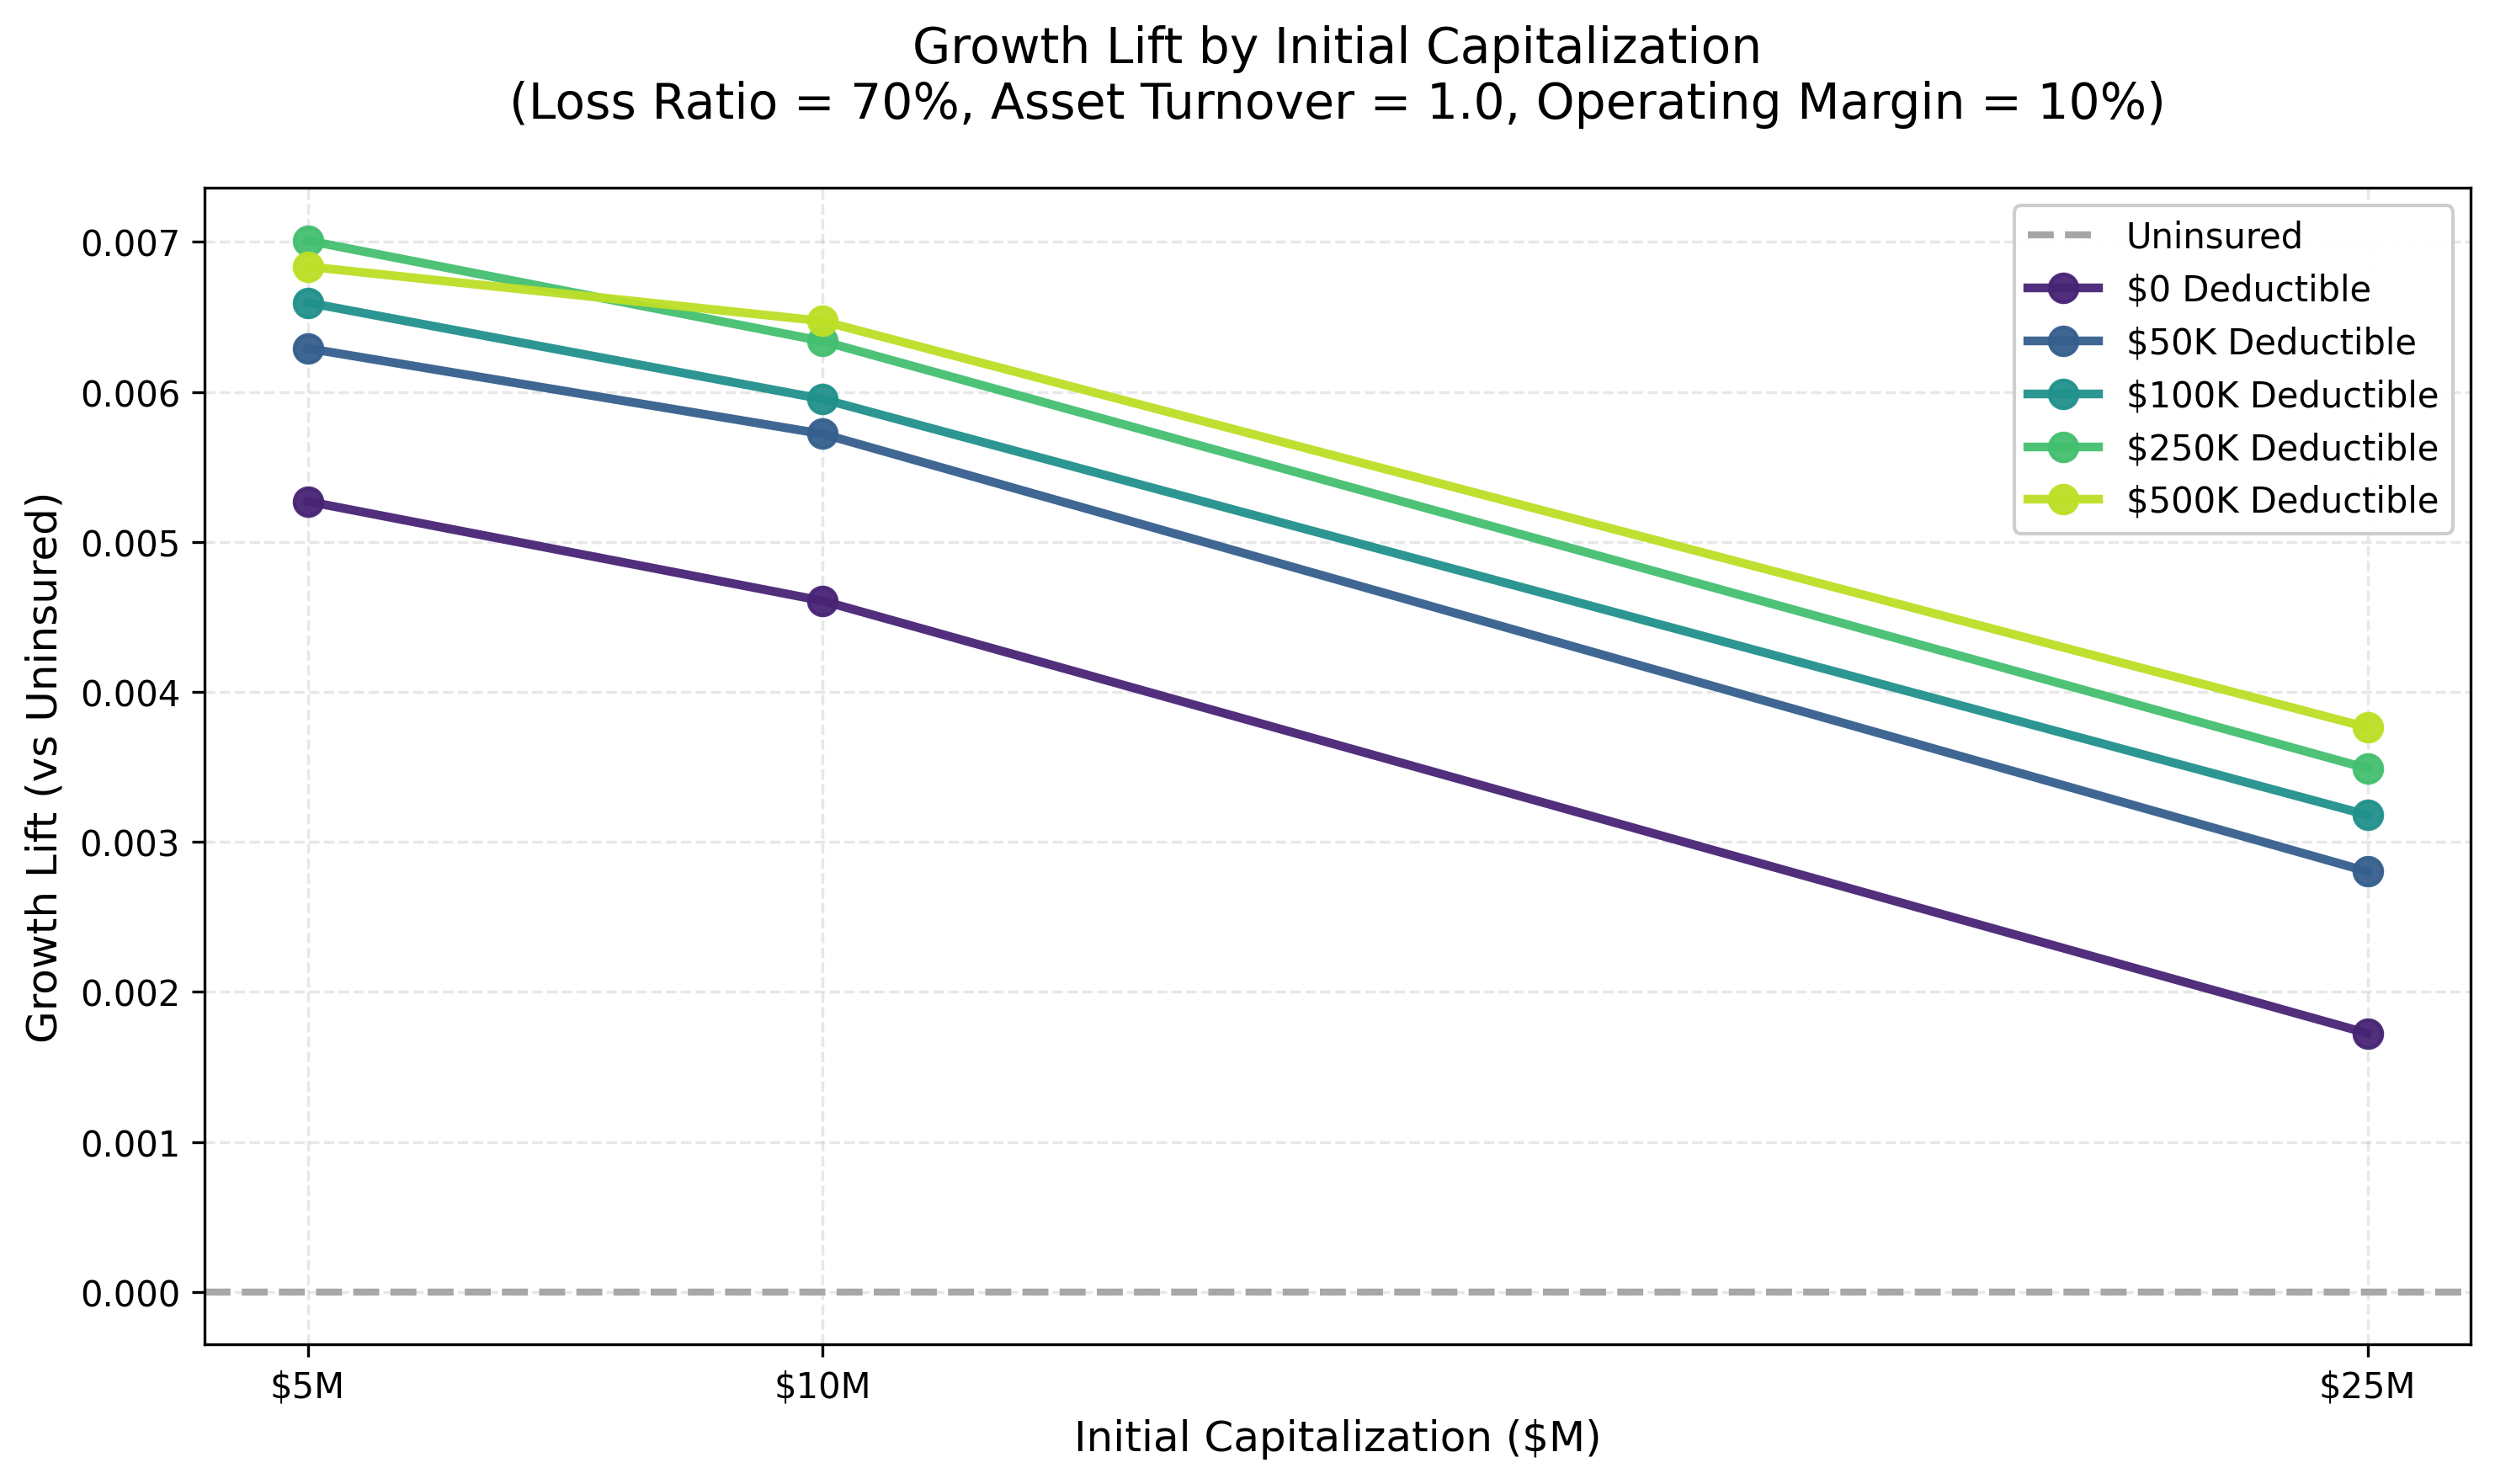
\includegraphics[width=1.0\textwidth]{images/growth_lift_by_capitalization.png}
    \caption{Impact of initial capitalization on time-average growth rate.}
    \label{fig:growth_lift_by_cap}
\end{figure}

\subsection{Operating Margin Interactions}

Operating margins serve to "flatten out" the growth lift across asset turnover ratios (ATR), which can be seen in Figures~\ref{fig:multiples_ebit_0.100}, \ref{fig:multiples_ebit_0.125}, and~\ref{fig:multiples_ebit_0.150}. This makes sense because both margin and ATR contribute to growth over time (ATR by generating revenue, and margins by retaining net income).

\subsection{Sensitivity to Insurance Pricing}

As expected, lower target loss ratios (i.e., cheaper insurance) increase the growth lift from insurance and shift optimal deductibles lower. However, even at relatively costly loss ratios of 60\%, insurance still provides substantial growth benefits at lower capitalizations. This finding challenges traditional views that insurance is a cost to be minimized. The ergodic perspective reveals that the multiplicative impact of catastrophic losses creates value in variance reduction that outweighs premium costs, particularly for smaller firms. Even at "expensive" loss ratio of 60\%, a firm with \$5M capitalization still does well with a low deductible of \$100K, and even \$50K deductibles and Guaranteed Cost provide substantial lift over self-insurance.

\begin{figure}[htbp]
    \centering
    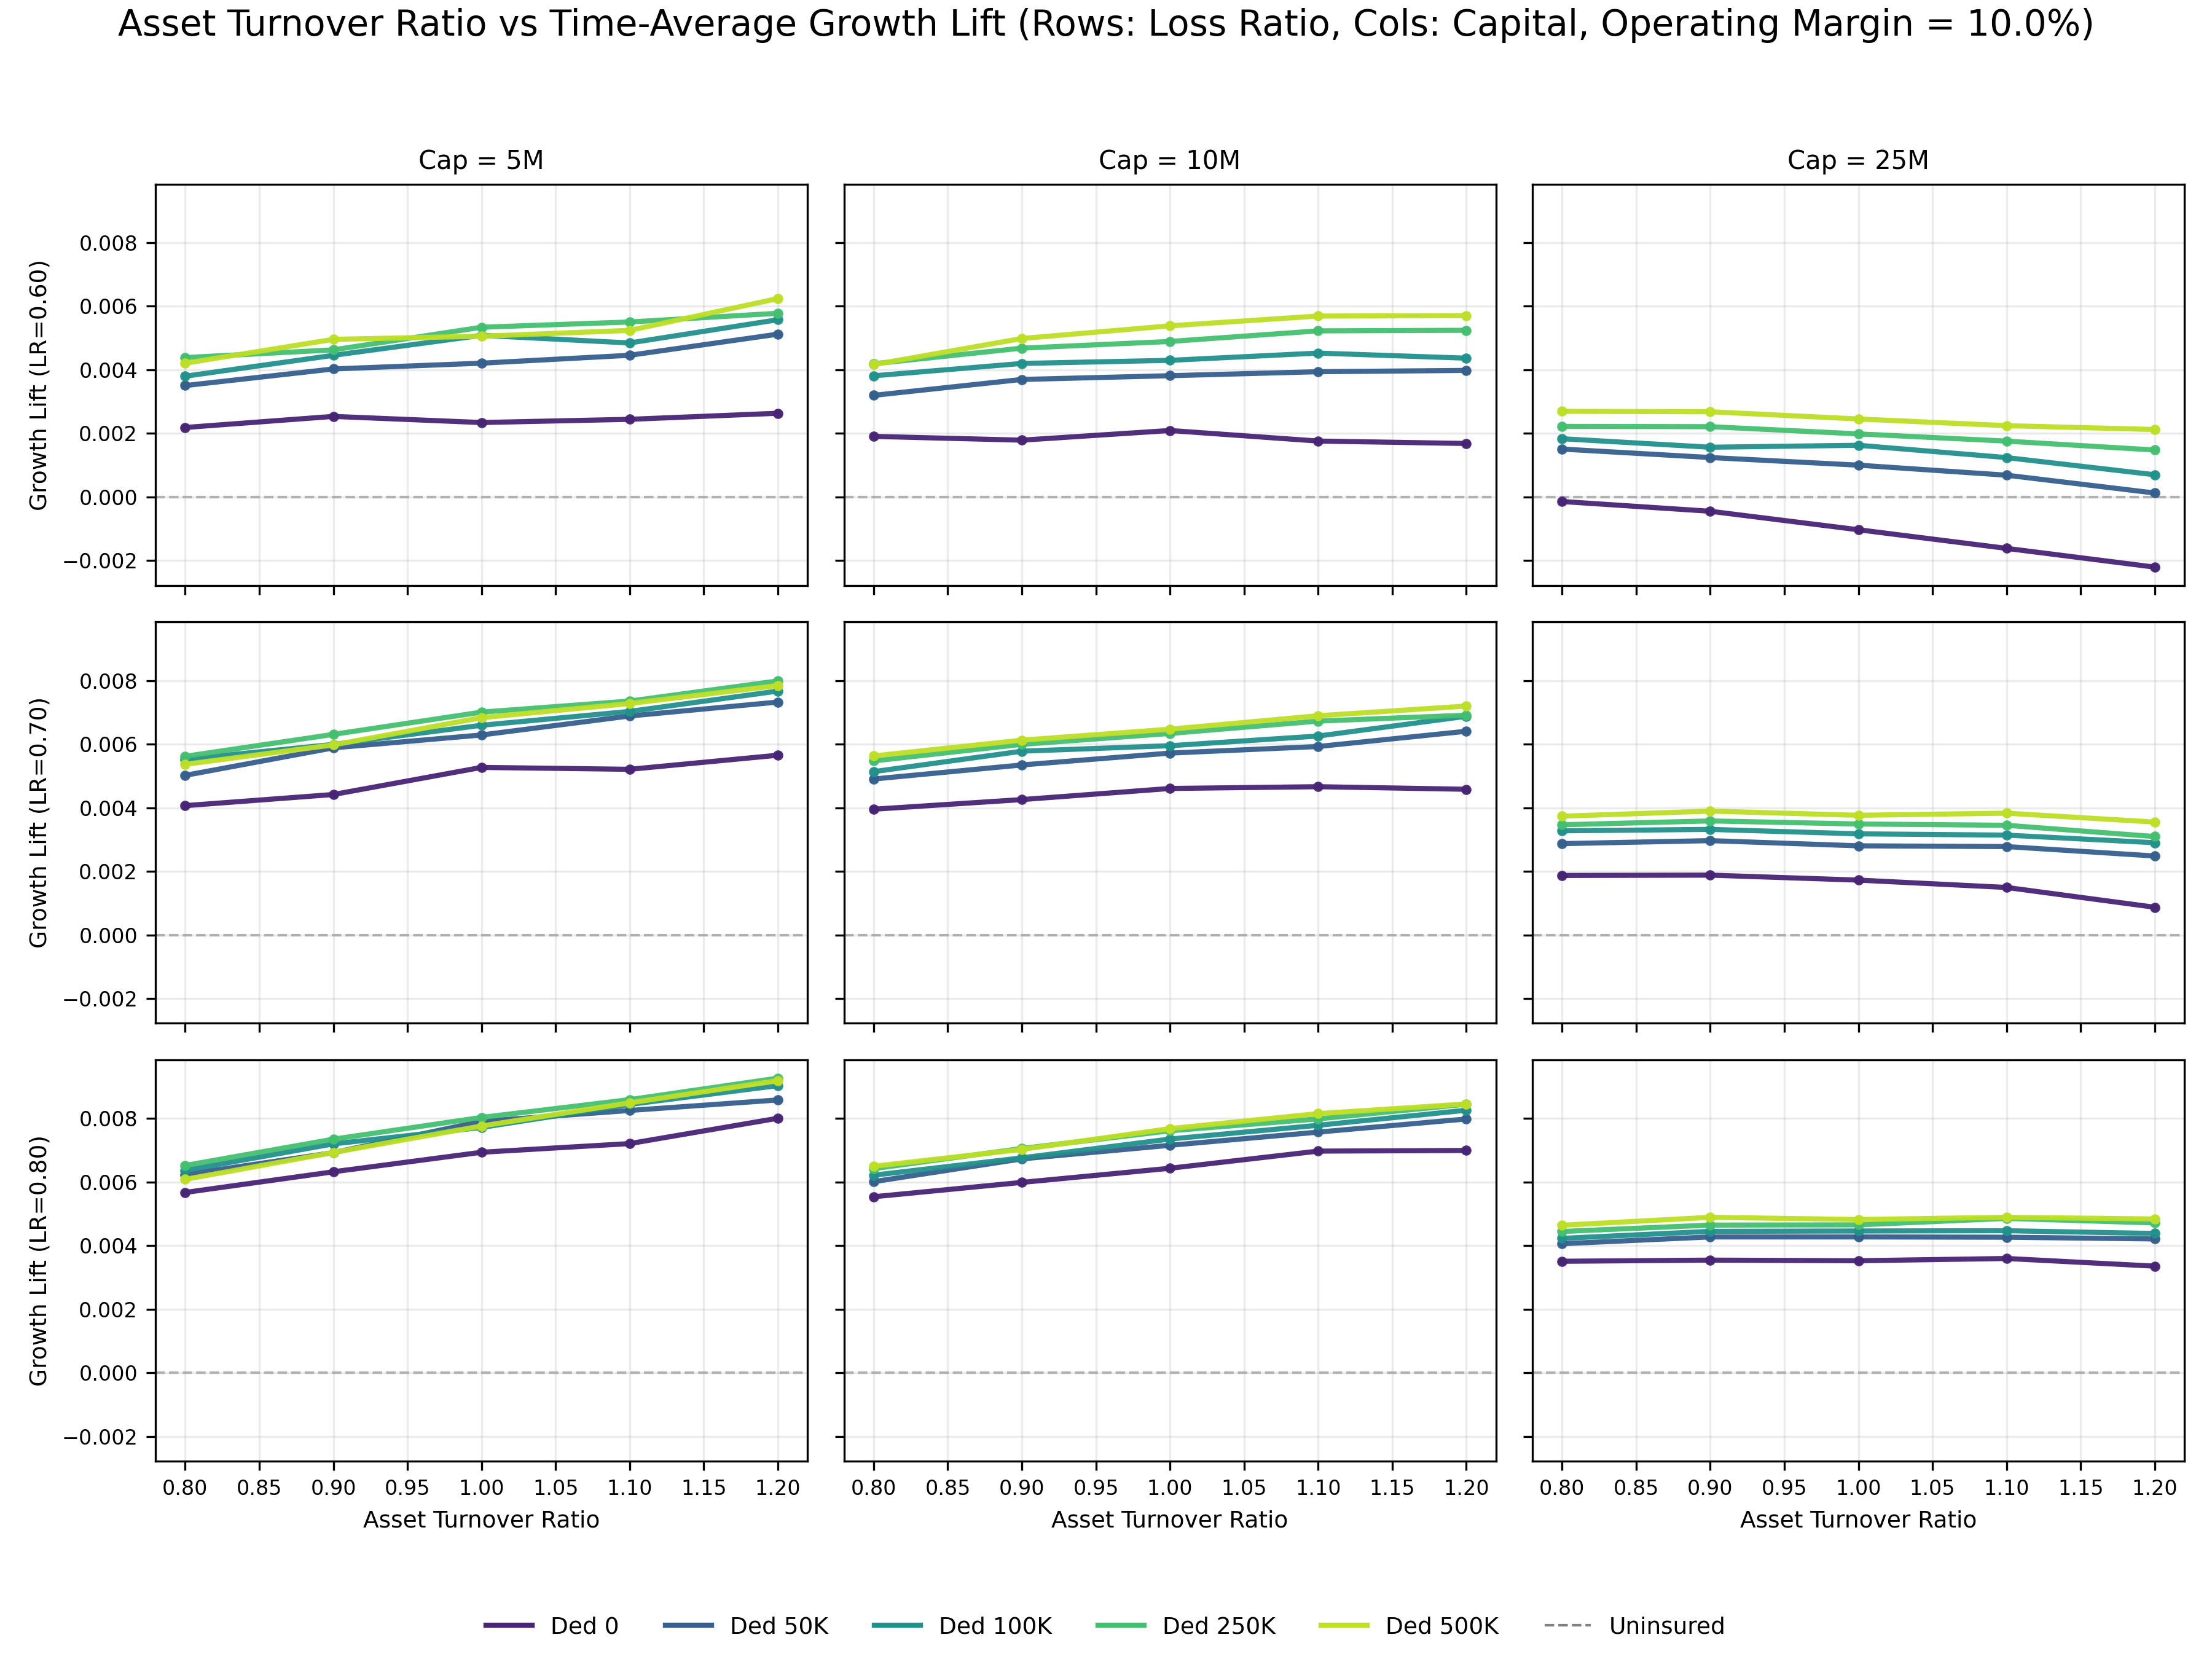
\includegraphics[width=1.0\textwidth]{images/option3_multiples_ebit_0.100.png}
    \caption{Impact of asset turnover ratio on time-average growth rate at operating margin of 10\%.}
    \label{fig:multiples_ebit_0.100}
\end{figure}

\begin{figure}[htbp]
    \centering
    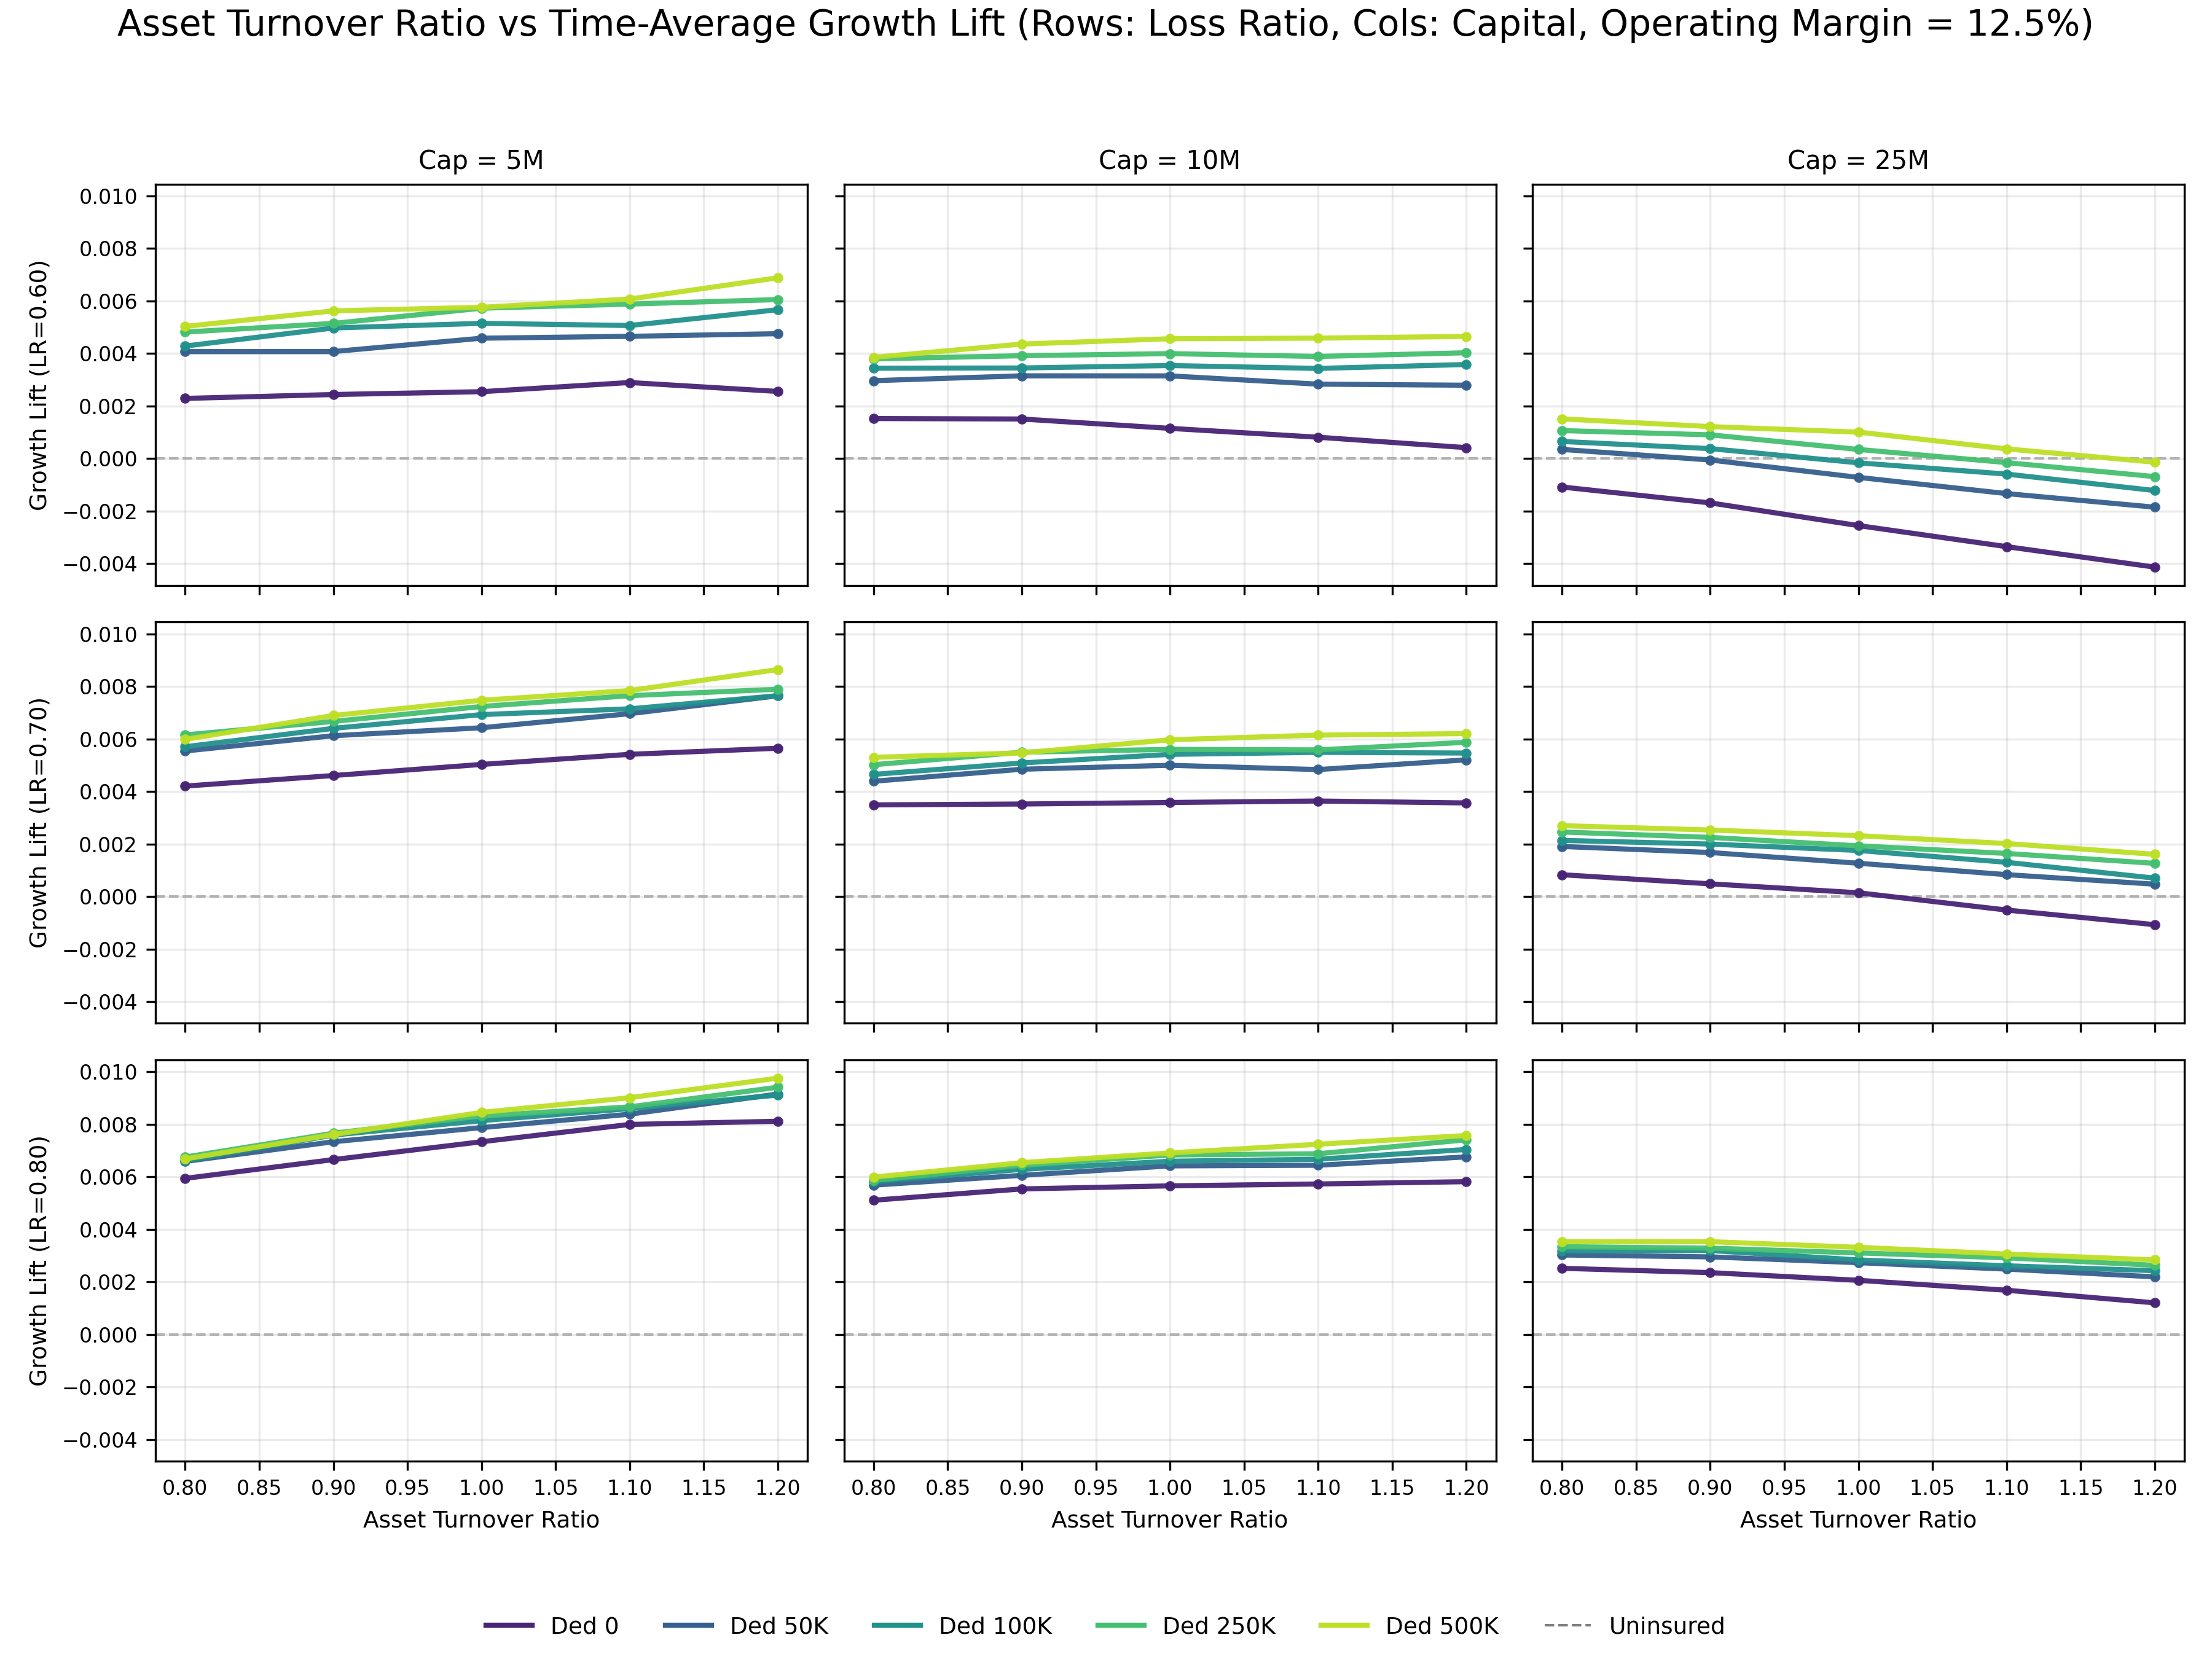
\includegraphics[width=1.0\textwidth]{images/option3_multiples_ebit_0.125.png}
    \caption{Impact of asset turnover ratio on time-average growth rate at operating margin of 12.5\%.}
    \label{fig:multiples_ebit_0.125}
\end{figure}

\begin{figure}[htbp]
    \centering
    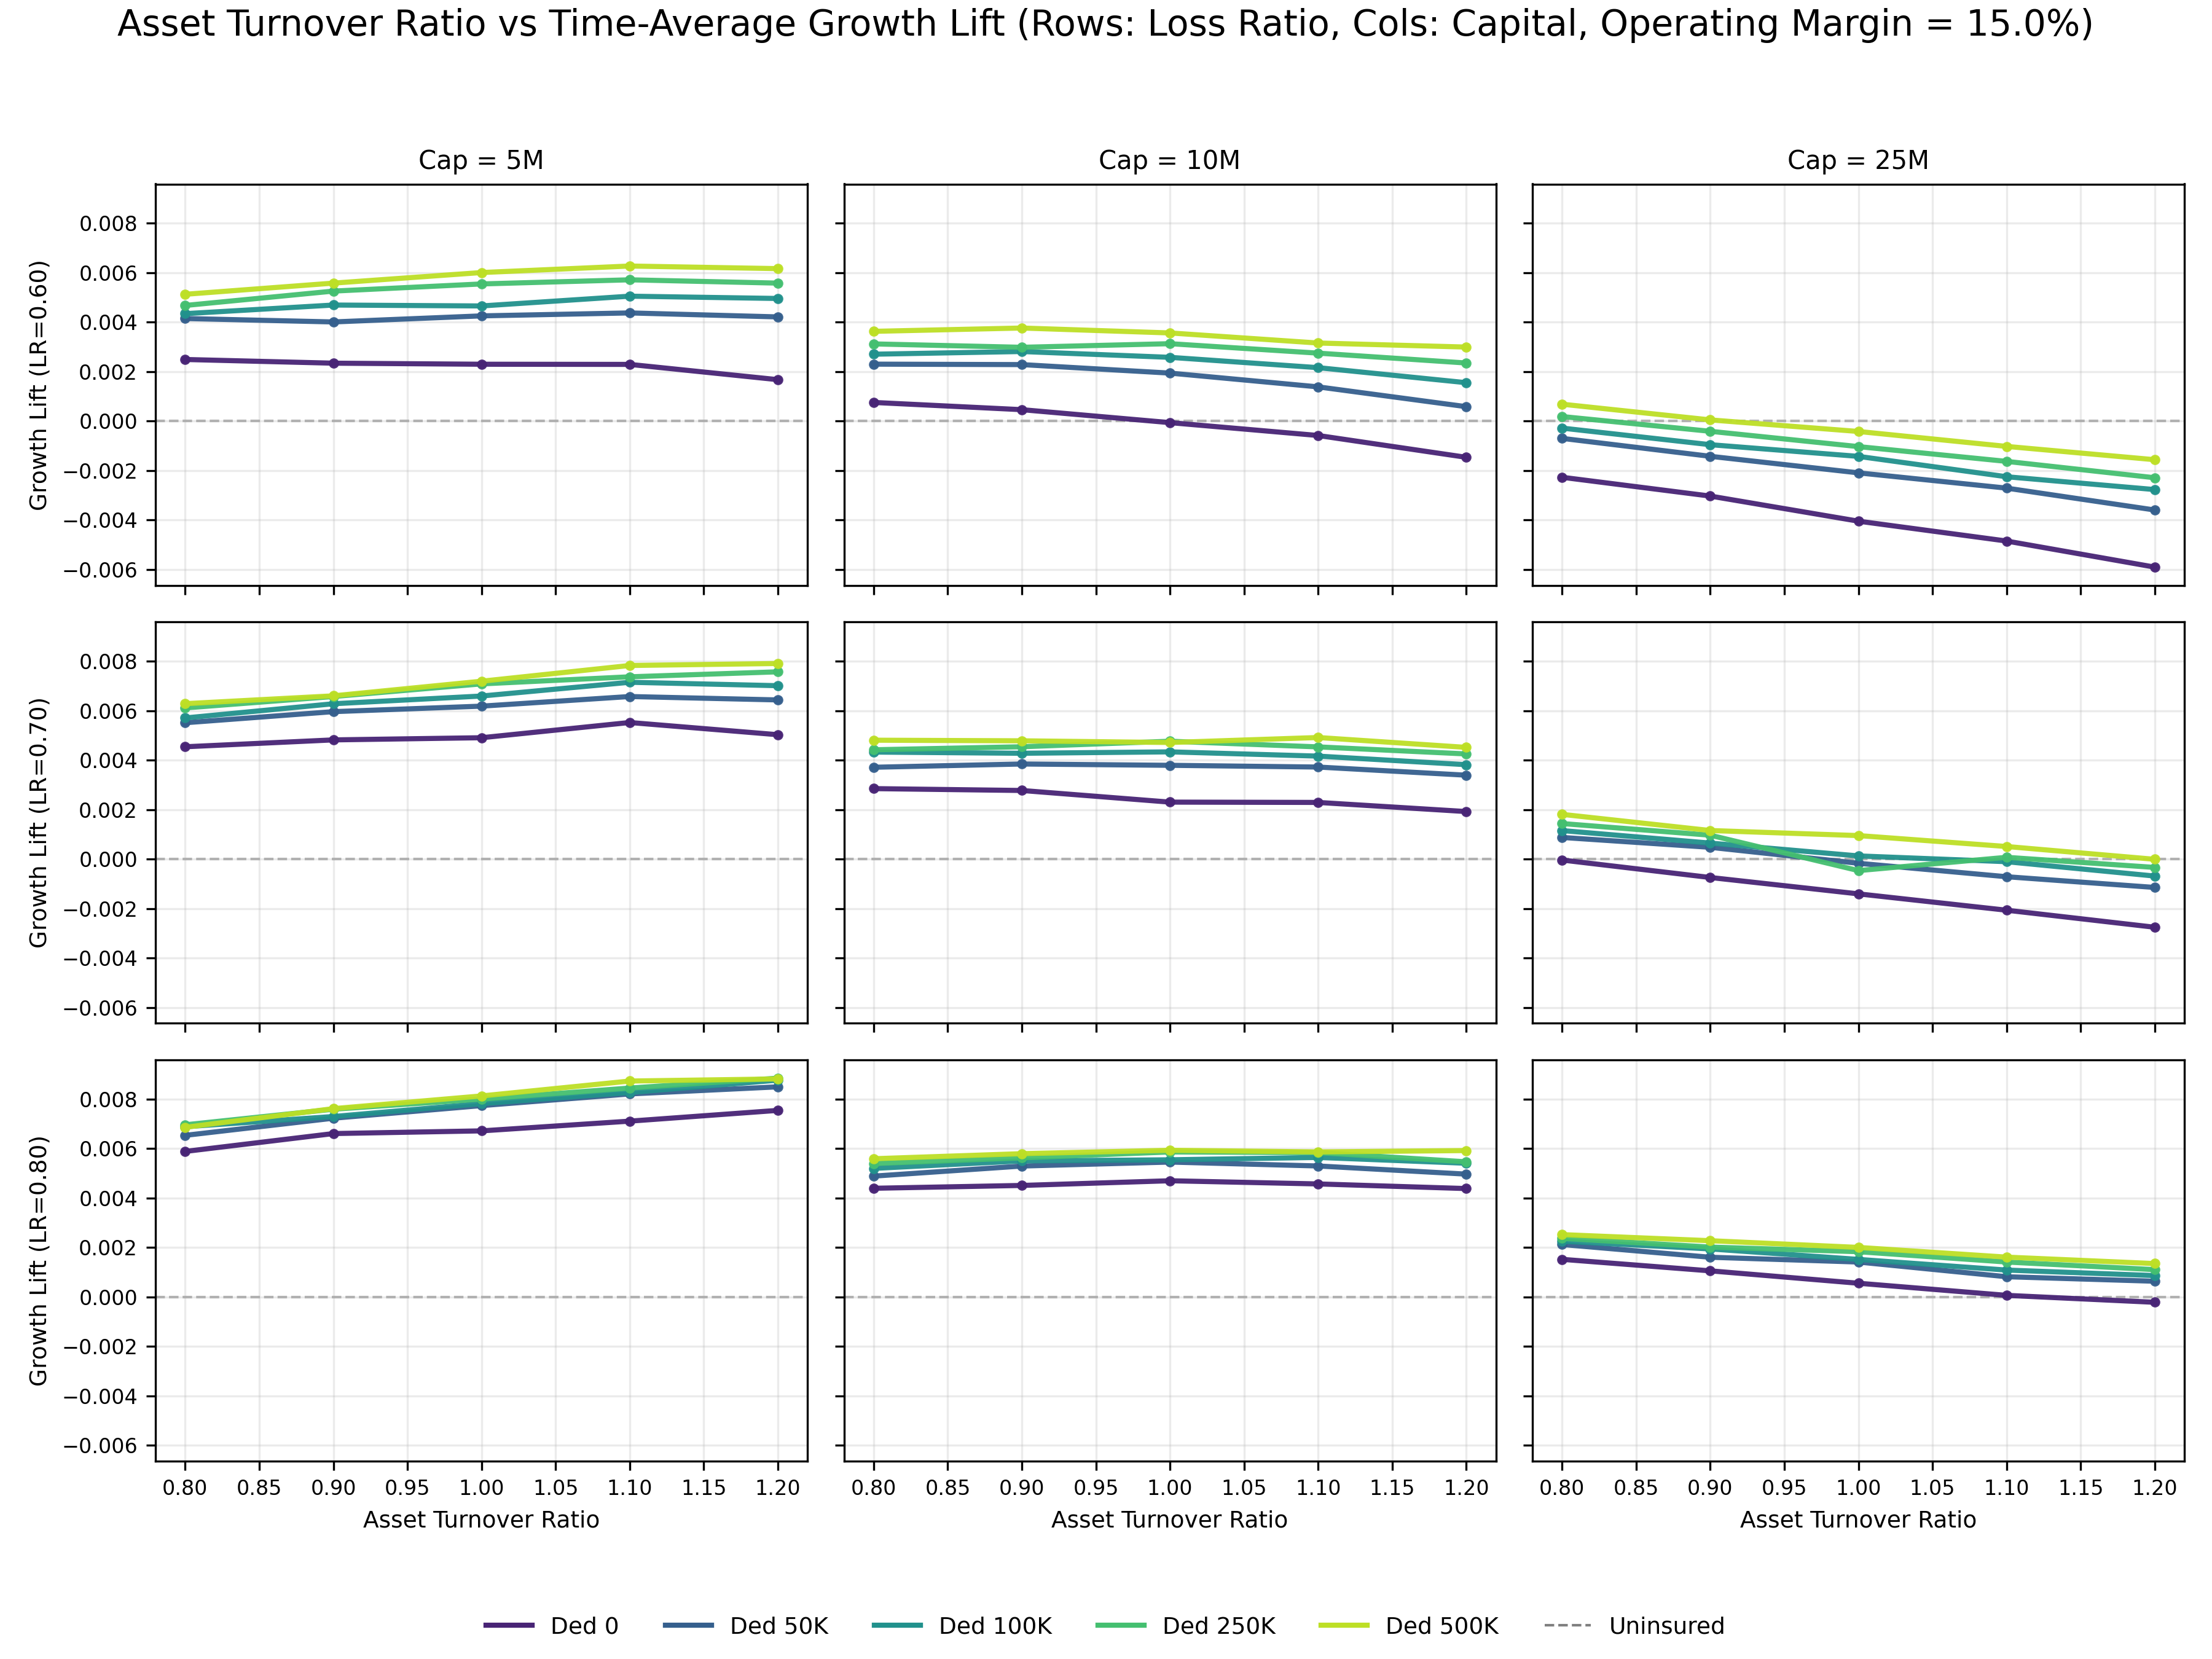
\includegraphics[width=1.0\textwidth]{images/option3_multiples_ebit_0.150.png}
    \caption{Impact of asset turnover ratio on time-average growth rate at operating margin of 15\%.}
    \label{fig:multiples_ebit_0.150}
\end{figure}

\section{Implications for Insurance Decision-Making}

\subsection{Reframing Insurance Value Through Time Averages}

The ergodic perspective fundamentally changes how corporate decision-makers should evaluate insurance. Rather than focusing on expected values and traditional cost-benefit analyses, risk managers must consider the time-average growth rate experienced by their specific company over its operational horizon. This shift reveals that insurance premiums substantially exceeding expected losses can still enhance long-term value creation by reducing the multiplicative impact of catastrophic events.

\subsection{The Ergodic Perspective on Risk Retention}

The simulation demonstrates that some level of risk retention is consistently optimal, challenging both full insurance and complete self-insurance strategies. This finding emerges from the ergodic framework's recognition that predictable attritional losses should be retained while catastrophic tail risks require transfer. The optimal retention level balances premium savings against the growth-destroying potential of large losses.

\subsection{Company Profile Considerations}

\textbf{Important Note:} The specific results presented in this paper are illustrative and depend heavily on the modeled loss distributions, business parameters, and simplifying assumptions. Corporate decision-makers should not apply these findings directly but rather use them as motivation to conduct company-specific ergodic analysis.

Key considerations emerging from the simulation include the critical role of capitalization levels, operating margin buffers, and loss severity distributions in determining optimal insurance strategies. Companies with lower capitalizations relative to potential losses derive substantially more value from insurance, even at higher premium rates.

\subsection{Engaging Actuarial Expertise for Ergodic Analysis}

CFOs and risk managers should engage experienced actuaries to model time-dependent paths specific to their industry and company characteristics. Traditional actuarial analysis focusing on expected values and ensemble statistics may systematically undervalue insurance for growth-focused companies. The actuarial profession must evolve to incorporate ergodic considerations into standard practice, developing new tools and methodologies for time-average optimization.

\subsection{Challenging Traditional Risk Management Metrics}

Standard risk metrics such as Value at Risk (VaR) and Expected Shortfall fail to capture the multiplicative nature of wealth dynamics and the critical distinction between time and ensemble averages. Risk management frameworks must evolve to incorporate ergodic considerations, particularly for long-term strategic decisions where path dependence and growth optimization matter more than short-term volatility measures.

\section{Future Research Directions}

This initial exploration of ergodic insurance optimization reveals numerous opportunities for extending the framework to address current model limitations and enhance practical applicability.

\subsection{Optimizing Complex Insurance Structures}

The current model's simplification to deductible-only structures masks important optimization opportunities in real-world insurance programs. Future research should incorporate:
\begin{itemize}
    \item Multi-layer tower structures with different attachment points and limits
    \item Aggregate deductibles and limits that recognize claim correlation
    \item Reinstatement provisions and their impact on tail risk protection
    \item Coverage sub-limits by peril or location
\end{itemize}

These extensions would enable practitioners to optimize complete insurance programs rather than single-parameter deductibles.

\subsection{Dynamic and Adaptive Insurance Strategies}

Static insurance decisions fail to capture the dynamic nature of business growth and market evolution. Future work should develop:
\begin{itemize}
    \item Adaptive strategies that adjust coverage as companies grow
    \item Market-responsive approaches that capitalize on insurance pricing cycles
    \item Path-dependent optimization recognizing that insurance decisions affect future growth trajectories
    \item Switching costs and multi-year contract considerations
\end{itemize}

\subsection{Incorporating Loss Correlations and Portfolio Effects}

The independence assumption for losses oversimplifies real risk landscapes. Extensions should model:
\begin{itemize}
    \item Correlation between different loss types and business lines
    \item Diversification benefits in multi-line enterprises
    \item Systemic risks and contagion effects
    \item Natural hedging opportunities within business portfolios
\end{itemize}

\subsection{Stochastic Business and Market Dynamics}

The deterministic revenue and margin assumptions limit the model's realism. Future research should incorporate:
\begin{itemize}
    \item Inflation, discounting, and time value of money
    \item Revenue volatility and its interaction with insurance value
    \item Economic cycles affecting both business performance and loss frequencies
    \item Insurance market cycles and their impact on optimal retention
    \item Competitive dynamics and market share considerations
\end{itemize}

\subsection{Industry-Specific Applications and Regulatory Considerations}

The generic manufacturing model requires specialization for practical implementation:
\begin{itemize}
    \item Industry-specific loss distributions and exposure bases
    \item Regulatory capital requirements and their optimization
    \item Rating agency considerations and cost of capital impacts
    \item Sector-specific risk factors (e.g., cyber for technology, liability for healthcare)
\end{itemize}

These extensions would transform the framework from an illustrative model to a practical decision support tool for corporate risk management.

\section{Conclusion}

This white paper has introduced a novel simulation framework based on ergodicity economics principles for analyzing insurance risk appetite. Our key findings demonstrate that company size significantly influences risk appetite, with larger insurers exhibiting greater willingness to underwrite risk. This finding has important implications for competitive dynamics and market structure in P\&C insurance.

The simulation framework provides a powerful tool for:
\begin{itemize}
    \item Understanding temporal risk dynamics
    \item Optimizing portfolio decisions
    \item Informing strategic planning
\end{itemize}

I encourage industry practitioners to explore these concepts further and welcome collaboration on extending this research.

The framework will provide new insights for companies making insurance decisions and is intended to answer questions such as "what is the ROI of our insurance program?", "how much insurance do we need?" and considerations of optimal insurance deductibles and limits.

% Bibliography
\bibliographystyle{apalike}
\bibliography{references}

\pagebreak

% Appendices
\appendix
\section{Technical Appendix}

\subsection{Simulation Algorithm Details}

This appendix provides algorithmic details for the core simulation engine, with emphasis on the timing of financial statement updates, insurance claim payments, and premium recognition. Readers interested in full implementation details should consult the GitHub repository referenced in Section~\ref{sec:code-repo}.

\subsubsection{Annual Simulation Loop}

The simulation executes a discrete-time loop over the specified horizon $T$ (50 years in this case), generating loss events and updating financial state at annual intervals. The high-level algorithm proceeds as follows:

\begin{algorithmic}[1]
\State \textbf{Initialize:} $t \gets 0$, Assets$_0 \gets$ initial capital, Equity$_0 \gets$ Assets$_0$
\State \textbf{Initialize:} Outstanding claims $\mathcal{C} \gets \emptyset$
\While{$t < T$ \textbf{and} Equity$_t > 0$}
    \State Generate loss events $L_t$ from three-tier loss distribution (see Section~\ref{sec:loss-gen})
    \For{each loss $\ell \in L_t$}
        \State Allocate $\ell$ between company retention and insurance recovery
        \State Create claim liability with 10-year payment schedule
        \State Post collateral for company portion: Collateral $\gets$ Collateral $+$ retention($\ell$)
    \EndFor
    \State Calculate revenue: $R_t \gets \text{Assets}_t \times \text{TurnoverRatio}$
    \State Calculate operating income: $\text{EBIT}_t \gets R_t \times \text{Margin} - \text{Premiums}_t - \text{Depreciation}_t \text{ (always 0)}$
    \State Process scheduled claim payments from $\mathcal{C}$ (Algorithm~\ref{alg:claim-payments})
    \State Calculate net income: $\text{NI}_t \gets (\text{EBIT}_t - \text{Losses}_t) \times (1 - \tau)$ \text{ (where } $\tau$ \text{ is the tax rate)}
    \State Update equity: Equity$_{t+1} \gets$ Equity$_t +$ NI$_t \times \rho$ (where $\rho$ is the retention ratio)
    \State Update assets: Assets$_{t+1} \gets$ Equity$_{t+1} +$ Liabilities$_{t+1}$
    \State $t \gets t + 1$
\EndWhile
\State \textbf{Return:} Time series $\{\text{Assets}_t, \text{Equity}_t, \text{Revenue}_t, \text{ROE}_t\}_{t=0}^{T}$
\end{algorithmic}

The simulation terminates upon insolvency (Equity$_t \leq 0$) or completion of the time horizon. The time-average growth rate for each trajectory is calculated as:
\begin{equation}
g_{\text{time}} = \frac{1}{T} \ln\left(\frac{\text{Equity}_T}{\text{Equity}_0}\right)
\end{equation}

This logarithmic formulation captures the multiplicative nature of wealth evolution and forms the basis for ergodic analysis across Monte Carlo scenarios.

\subsubsection{Balance Sheet Update Mechanism}

The annual \texttt{step()} method orchestrates financial statement updates with careful attention to the sequence of operations. The order is critical because each calculation affects subsequent balance sheet items. The method follows this sequence:

\begin{algorithmic}[1]
\State \textbf{Input:} Current balance sheet state, working capital percentage $w$, LoC rate $r_{\text{LoC}}$
\State \textbf{Step 1: Revenue Calculation}
\State Adjust for working capital: $A_{\text{eff}} \gets \frac{\text{Assets}}{1 + \text{Turnover} \times w}$ \text{ (}$w$ \text{is 0\% in this experiment)}
\State Calculate revenue: $R \gets A_{\text{eff}} \times \text{TurnoverRatio}$
\State \textbf{Step 2: Operating Income}
\State Calculate base operating income: $\text{EBIT}_{\text{base}} \gets R \times \text{OperatingMargin}$
\State Subtract insurance premiums: $\text{EBIT} \gets \text{EBIT}_{\text{base}} - \text{Premiums}$
\State Subtract depreciation: $\text{EBIT} \gets \text{EBIT} - \text{Depreciation (0 in this experiment)}$
\State \textbf{Step 3: Claim Payments and Collateral}
\State Process scheduled payments: \{payments, collateral released\} $\gets$ \texttt{pay\_claim\_liabilities()}
\State Accrue letter of credit charges: $\text{LoC\_cost} \gets \text{Collateral} \times r_{\text{LoC}}$
\State Record insurance losses for tax purposes: $\text{LossesPaid} \gets$ sum(payments)
\State \textbf{Step 4: Net Income}
\State Taxable income: $\text{TI} \gets \text{EBIT} - \text{LossesPaid} - \text{LoC\_cost}$
\State Net income: $\text{NI} \gets \text{TI} \times (1 - \tau)$
\State \textbf{Step 5: Balance Sheet Update}
\State Retained earnings: $\text{RE} \gets \text{NI} \times \rho$
\State Update equity: Equity$_{\text{new}} \gets$ Equity$_{\text{old}} + \text{RE}$
\State Update assets: Assets$_{\text{new}} \gets$ Equity$_{\text{new}} + $ Liabilities
\State \textbf{Return:} Metrics dictionary \{assets, equity, roe, revenue, net\_income, ...\}
\end{algorithmic}

\vspace{\baselineskip}

Key equations implemented in this sequence:

\vspace{\baselineskip}

\textbf{Operating Income:}
\begin{equation}
\text{EBIT} = R \times m - \text{Premiums} - \text{Depreciation}
\end{equation}
where $m$ is the base operating margin. Insurance premiums are treated as operating expenses, consistent with their role in the core business model.

\vspace{\baselineskip}

\textbf{Net Income and Equity Growth:}
\begin{equation}
\text{Equity}_{t+1} = \text{Equity}_t + (\text{EBIT}_t - \text{LossesPaid}_t - \text{LoC\_cost}_t) \times (1-\tau) \times \rho
\end{equation}
where $\tau$ is the corporate tax rate and $\rho$ is the earnings retention ratio. This formulation ensures that insurance losses receive proper tax treatment and that growth is funded entirely through retained earnings (no external capital).

\subsubsection{Claim Incurrence versus Payment Timing}

A critical feature of the simulation is the temporal separation between claim incurrence and claim payment. This distinction creates realistic cash flow dynamics and collateral requirements that fundamentally affect company liquidity and growth trajectories.

\vspace{\baselineskip}

\textbf{At Claim Incurrence (Year $t$):}

When a loss event occurs, the simulation immediately:
\begin{enumerate}
    \item Creates a claim liability for the company's portion (deductible):

        $L_{\text{company}} = \min(\text{Deductible}, \text{ClaimAmount})$

    \item Posts collateral via Letter of Credit: Collateral$_t \gets$ Collateral$_{t-1} + L_{\text{company}}$
    \item Records the liability on the balance sheet: Liabilities$_t \gets$ Liabilities$_{t-1} + L_{\text{company}}$
    \item Restricts assets equal to collateral: RestrictedAssets$_t \gets$ Collateral$_t$
\end{enumerate}

Critically, \textbf{no cash leaves the company} at claim incurrence. Instead, assets are restricted and begin accruing Letter of Credit charges at rate $r_{\text{LoC}}$ (here, 1.5\% annually):
\begin{equation}
\text{LoC Cost}_t = \text{Collateral}_t \times r_{\text{LoC}}
\end{equation}

\textbf{During Payment Period (Years $t$ through $t+9$):}

Each year, the simulation processes scheduled payments according to the claim development pattern:
\begin{enumerate}
    \item Calculate payment due: $\text{Payment}_{\tau} = L_{\text{company}} \times d_{\tau-t}$ where $d_k$ is the development factor for year $k$
    \item Reduce cash: Cash $\gets$ Cash $-$ Payment$_{\tau}$
    \item Reduce liability: Liability $\gets$ Liability $-$ Payment$_{\tau}$
    \item Release collateral: Collateral $\gets$ Collateral $-$ Payment$_{\tau}$
    \item Release restricted assets: RestrictedAssets $\gets$ Collateral
\end{enumerate}

This creates an asymmetric cash flow profile: \textbf{immediate collateral requirement and ongoing LoC costs, but gradual cash outflow}. The restricted assets cannot be used for operations, reducing available capital for revenue generation:
\begin{equation}
\text{AvailableAssets}_t = \text{TotalAssets}_t - \text{RestrictedAssets}_t
\end{equation}

\textbf{Balance Sheet Impact:}

The accounting identity Assets $=$ Liabilities $+$ Equity is maintained throughout, but the composition changes over the payment period:

\begin{center}
\begin{tabular}{lcc}
\toprule
\textbf{Balance Sheet Item} & \textbf{At Incurrence} & \textbf{Over Payment Period} \\
\midrule
Cash & No change & Decreases gradually \\
Restricted Assets & Increases & Decreases gradually \\
Total Assets & No change & Decreases gradually \\
Claim Liabilities & Increases & Decreases gradually \\
Equity & No change* & Affected by LoC costs \\
\bottomrule
\multicolumn{3}{l}{\small *Equity unchanged at incurrence; LoC costs reduce it over time}
\end{tabular}
\end{center}

This temporal structure is fundamental to the model's realism. It captures the actuarial reality that claim liabilities are recognized immediately when the insured event occurs (accrual accounting), but cash settlements follow a protracted schedule driven by investigation, negotiation, litigation, and payment processing.

\subsubsection{Multi-Year Claim Payment Schedule}
\label{alg:claim-payments}

Claims follow a standardized 10-year development pattern representing typical long-tail liability settlement, calibrated to general liability and manufacturing claims experience:

\begin{equation}
\mathbf{d} = [0.10, 0.20, 0.20, 0.15, 0.10, 0.08, 0.07, 0.05, 0.03, 0.02]
\end{equation}

where $d_k$ is the percentage of the original claim paid in year $k$ (zero-indexed from year of incurrence). This pattern reflects several actuarial features:
\begin{itemize}
    \item \textbf{Front-loaded payments} (40\% in first two years): Initial payments for clear-cut liability
    \item \textbf{Peak in year 2-3} (20\% each): Settlement of straightforward cases
    \item \textbf{Gradual tail} (years 4-10): Complex litigation, structured settlements, late-developing injuries
\end{itemize}

The implementation in \texttt{ClaimLiability.get\_payment()} calculates payments for any claim in any year:

\begin{lstlisting}[language=Python, caption={Claim Payment Calculation}, label={lst:claim-payment}]
def get_payment(self, years_since_incurred: int) -> float:
    """Calculate payment due for a given year after claim incurred."""
    if years_since_incurred < 0 or
       years_since_incurred >= len(self.payment_schedule):
        return 0.0
    return self.original_amount * self.payment_schedule[years_since_incurred]
\end{lstlisting}

Each simulation year, all outstanding claims are processed collectively:

\begin{lstlisting}[language=Python, caption={Annual Claim Payment Processing (simplified)}, label={lst:pay-claims}]
def pay_claim_liabilities(self) -> Dict[str, float]:
    """Process scheduled payments for all outstanding claims."""
    total_paid = 0.0
    collateral_released = 0.0

    for claim in self.claim_liabilities:
        years_elapsed = self.current_year - claim.year_incurred
        scheduled_payment = claim.get_payment(years_elapsed)

        # Make payment and release collateral
        actual_payment = claim.make_payment(scheduled_payment)
        total_paid += actual_payment
        collateral_released += actual_payment

    # Update balance sheet
    self.cash -= total_paid
    self.collateral -= collateral_released
    self.restricted_assets = self.collateral

    # Remove fully paid claims
    self.claim_liabilities = [c for c in self.claim_liabilities
                             if c.remaining_amount > 0]

    return {"total_paid": total_paid, "collateral_released": collateral_released}
\end{lstlisting}

This approach efficiently handles overlapping claim cohorts: a company may have dozens of claims at various stages of development, each following its own schedule. The collateral balance equals the sum of remaining liabilities across all active claims:
\begin{equation}
\text{Collateral}_t = \sum_{c \in \mathcal{C}_t} \text{RemainingLiability}_c
\end{equation}
where $\mathcal{C}_t$ is the set of active claims at time $t$.

\subsubsection{Premium Payment and Expense Recognition}

Insurance premiums follow a simplified timing structure that balances realism with computational efficiency:

\vspace{\baselineskip}

\textbf{Premium Calculation:} Premiums are calculated once at simulation inception based on the expected loss distribution and target loss ratio:
\begin{equation}
\text{Premium}_0 = \frac{\E[L]_0}{\text{LossRatio}_{\text{target}}}
\end{equation}

where $\E[L]_0$ is the expected annual loss at initial revenue level, estimated via a separate Monte Carlo simulation with 500,000 pricing runs. Typical target loss ratios are 60\%, 70\%, or 80\%, representing varying degrees of insurer expense loading and profit margin.

\vspace{\baselineskip}

\textbf{Revenue Scaling:} In subsequent years, premiums scale proportionally with revenue to maintain constant coverage relative to exposure:
\begin{equation}
\text{Premium}_t = \text{Premium}_0 \times \frac{\text{Revenue}_t}{\text{Revenue}_0}
\end{equation}

This reflects the reality that insurance pricing adjusts to changing exposure bases, which in this case is revenue, though it is simplified by omitting experience rating, market cycles, and multi-year policy structures (extensions for future research).

\vspace{\baselineskip}

\textbf{Expense Recognition:} Premiums are recorded as operating expenses in the year incurred, directly reducing EBIT:
\begin{equation}
\text{EBIT}_t = \text{Revenue}_t \times \text{Margin} - \text{Premium}_t - \text{Depreciation}_t
\end{equation}

This treatment is consistent with the simulation's annual time resolution. More sophisticated implementations could incorporate:
\begin{itemize}
    \item \textbf{Prepaid insurance assets} for annual policies paid in advance, with monthly amortization
    \item \textbf{Premium accruals} for policies with different payment schedules (quarterly, annual)
    \item \textbf{Multi-year policies} with premium smoothing and experience-based adjustments
\end{itemize}

The current implementation trades this complexity for computational speed and conceptual clarity, focusing the analysis on the core ergodic question: how do deductible choices affect long-term growth rates?

\vspace{\baselineskip}

\textbf{Tax Treatment:} Premiums are fully deductible in the year paid, reducing taxable income dollar-for-dollar:
\begin{equation}
\text{TaxBenefit}_t = \text{Premium}_t \times \tau
\end{equation}
where $\tau = 0.25$ is the corporate tax rate. This partially offsets premium costs, making insurance more attractive on an after-tax basis, which is properly captured in the net income calculation.

\subsubsection{Loss Generation Process}
\label{sec:loss-gen}

The simulation employs a three-tier loss structure that captures the full spectrum of operational risks facing a manufacturing company. Each tier uses a compound Poisson process where claim counts and severities are independently drawn from calibrated distributions.

\vspace{\baselineskip}

\textbf{Tier 1: Attritional Losses}

High-frequency, low-severity events such as minor equipment failures, small liability claims, and routine operational disruptions. Parameters:
\begin{align}
N_{\text{att}} &\sim \text{Poisson}(\lambda_{\text{att}}) \quad \text{where } \lambda_{\text{att}} = 2.85 \times \frac{R_t}{R_0} \\
X_{\text{att}} &\sim \text{Lognormal}(\mu = \$40\text{K}, \text{CV} = 0.8)
\end{align}

The revenue scaling factor $R_t / R_0$ ensures claim frequency grows with business exposure.

\vspace{\baselineskip}

\textbf{Tier 2: Large Losses}

Moderate-frequency events with substantial impact, including significant equipment breakdowns, supply chain disruptions, and major liability claims. Parameters:
\begin{align}
N_{\text{large}} &\sim \text{Poisson}(\lambda_{\text{large}}) \quad \text{where } \lambda_{\text{large}} = 0.20 \times \frac{R_t}{R_0} \\
X_{\text{large}} &\sim \text{Lognormal}(\mu = \$500\text{K}, \text{CV} = 1.5)
\end{align}

\vspace{\baselineskip}

\textbf{Tier 3: Catastrophic Losses}

Low-probability, high-impact events that threaten business continuity, such as natural disasters, major litigation, or systemic failures. Parameters:
\begin{align}
N_{\text{cat}} &\sim \text{Poisson}(\lambda_{\text{cat}}) \quad \text{where } \lambda_{\text{cat}} = 0.02 \times \frac{R_t}{R_0} \\
X_{\text{cat}} &\sim \text{Pareto}(x_{\text{min}} = \$5\text{M}, \alpha = 1.5)
\end{align}

The Pareto distribution for catastrophic losses creates heavy-tailed risk: losses can be arbitrarily large, though with rapidly declining probability. This captures the fundamental uncertainty in extreme events that drives much of the insurance value proposition.

\vspace{\baselineskip}

\textbf{Total Annual Losses:}
\begin{equation}
L_t = \sum_{i=1}^{N_{\text{att}}(t)} X_{\text{att}}^{(i)} + \sum_{j=1}^{N_{\text{large}}(t)} X_{\text{large}}^{(j)} + \sum_{k=1}^{N_{\text{cat}}(t)} X_{\text{cat}}^{(k)}
\end{equation}

All loss counts are independent across tiers and years. Claim amounts are drawn independently, and no correlation is modeled between loss types or between losses and business performance (beyond the revenue exposure scaling). These simplifications enhance computational efficiency while maintaining the essential features of manufacturing risk profiles. See Section~3.2 for complete parameter specifications and calibration rationale.

\subsection{Code Repository}\label{sec:code-repo}

The GitHub repository at \url{https://github.com/AlexFiliakov/Ergodic-Insurance-Limits}\\
contains the complete implementation, including additional features such as:
\begin{itemize}
    \item Stochastic revenue and margin processes for enhanced realism
    \item Regulatory capital requirements and rating agency constraints
    \item Multi-layer insurance tower optimization
    \item Parallel Monte Carlo execution with checkpoint/resume capability
    \item Comprehensive visualization and sensitivity analysis tools
\end{itemize}

\end{document}
